\documentclass{article}
\usepackage[preprint]{neurips_2024}
\usepackage{amsmath,amssymb}
\usepackage{booktabs}
\usepackage{graphicx}
\usepackage{hyperref}
\usepackage{algorithm}
\usepackage{algorithmic}
\usepackage{placeins}
\usepackage{tikz}
\usetikzlibrary{positioning,arrows.meta,calc,fit}

\newcommand{\vk}{\mathbf{k}}
\newcommand{\vv}{\mathbf{v}}
\newcommand{\vq}{\mathbf{q}}
\newcommand{\vx}{\mathbf{x}}
\newcommand{\vy}{\mathbf{y}}
\newcommand{\mW}{\mathbf{W}}
\newcommand{\mM}{\mathbf{M}}

\title{Memory Is All You Need}

\author{
  Jeff Guan \\
  \texttt{jeff.guan0@gmail.com}
}

\begin{document}
\maketitle

\begin{abstract}
Transformers and state space models (e.g.\ Mamba) use sophisticated mechanisms to mix information across sequence positions. We argue that \textbf{a minimal mixing backbone and an associative memory is all that is necessary}. We augment language models with a Hebbian memory---a matrix of outer-product associations updated at each token---and systematically ablate the backbone. \textbf{[TODO: update with final numbers]} On code generation: Mamba + Hebbian memory achieves 1.85 nats; replacing Mamba's recurrence with a 4-token depthwise convolution gives 1.94 nats at half the parameters; removing the backbone entirely still converges. The sequence model backbone contributes only local feature extraction; \textbf{the associative memory handles all long-range recall}.
\end{abstract}

\section{Introduction}

Transformers~\citep{vaswani2017attention} and state space models like Mamba~\citep{gu2024mamba,dao2024mamba2} use complex mechanisms---quadratic attention, selective gating, discretized recurrence---to capture long-range dependencies in sequences.

But what if associative memory, not the sequence model, is the primary mechanism for long-range reasoning? In this work, we decompose language modeling into two capabilities: first, \textbf{associative binding}---storing and retrieving associations across arbitrary distances---and second, \textbf{local feature extraction}---combining adjacent tokens into useful representations.

A Hebbian associative memory~\citep{hebb1949organization}---a decaying outer-product matrix updated at each token---handles the first entirely. For the second, a depthwise convolution over just 4 tokens suffices. The resulting architecture contains no recurrence, no attention, and no gating beyond SiLU, yet matches SSM-based models at comparable parameter counts.

Our key finding is stark: replacing Mamba with a 4-token convolution \textbf{[TODO: conv results pending]} matches performance at a fraction of the complexity, and a model with \emph{no} sequence mixing at all (pure linear projection + Hebbian) still converges to 3.18 nats. 

The associative memory is not merely an augmentation---it is retrieval and computation in one mechanism. It \emph{is} the model.

\section{Method}

\begin{figure}[t]
\centering
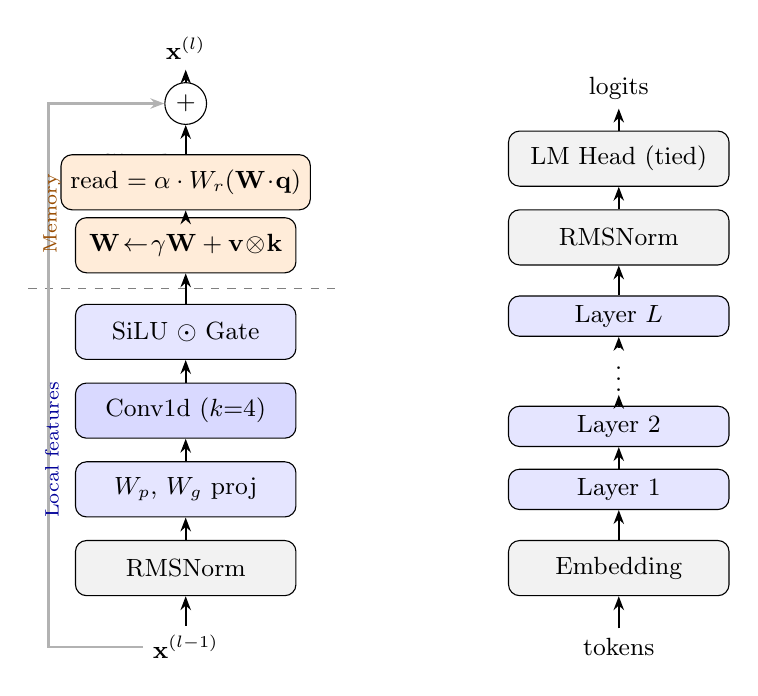
\begin{tikzpicture}[
    block/.style={draw, rounded corners, minimum width=2.8cm, minimum height=0.7cm, align=center, font=\small},
    op/.style={draw, circle, inner sep=2pt, font=\small},
    arr/.style={-{Stealth[length=5pt]}, thick},
    every node/.style={font=\small},
]
% === Single Layer (left) ===
\node[font=\normalsize\bfseries] at (0, 5.8) {Single Layer};

\node (in) at (0, -0.3) {$\vx^{(l-1)}$};
\node[block, fill=gray!10] (norm) at (0, 0.7) {RMSNorm};
\node[block, fill=blue!10] (proj) at (0, 1.7) {$W_p$, $W_g$ proj};
\node[block, fill=blue!15] (conv) at (0, 2.7) {Conv1d ($k{=}4$)};
\node[block, fill=blue!10] (gate) at (0, 3.7) {SiLU $\odot$ Gate};

% Divider
\draw[dashed, gray] (-2, 4.25) -- (2, 4.25);

\node[block, fill=orange!15] (write) at (0, 4.8) {$\mW \!\leftarrow\! \gamma\mW + \vv\!\otimes\!\vk$};
\node[block, fill=orange!15] (read) at (0, 5.6) {read $= \alpha \cdot W_r(\mW \!\cdot\! \vq)$};

\node[op] (add) at (0, 6.6) {$+$};
\node (out) at (0, 7.3) {$\vx^{(l)}$};

\draw[arr] (in) -- (norm);
\draw[arr] (norm) -- (proj);
\draw[arr] (proj) -- (conv);
\draw[arr] (conv) -- (gate);
\draw[arr] (gate) -- (write);
\draw[arr] (write) -- (read);
\draw[arr] (read) -- (add);
\draw[arr] (add) -- (out);

% Residual
\draw[arr, gray!60] (in.west) -- ++(-1.2,0) |- (add.west);

% Labels
\node[font=\scriptsize, blue!60!black, rotate=90] at (-1.7, 2.2) {Local features};
\node[font=\scriptsize, orange!60!black, rotate=90] at (-1.7, 5.2) {Memory};

% === Full Stack (right) ===
\node[font=\normalsize\bfseries] at (5.5, 5.8) {Full Model};

\node (emb_in) at (5.5, -0.3) {tokens};
\node[block, fill=gray!10] (emb) at (5.5, 0.7) {Embedding};

\node[block, fill=blue!10, minimum height=0.5cm] (l1) at (5.5, 1.7) {Layer 1};
\node[block, fill=blue!10, minimum height=0.5cm] (l2) at (5.5, 2.5) {Layer 2};
\node at (5.5, 3.2) {$\vdots$};
\node[block, fill=blue!10, minimum height=0.5cm] (lL) at (5.5, 3.9) {Layer $L$};

\node[block, fill=gray!10] (fnorm) at (5.5, 4.9) {RMSNorm};
\node[block, fill=gray!10] (head) at (5.5, 5.9) {LM Head (tied)};
\node (logits) at (5.5, 6.8) {logits};

\draw[arr] (emb_in) -- (emb);
\draw[arr] (emb) -- (l1);
\draw[arr] (l1) -- (l2);
\draw[arr] (l2) -- ++(0, 0.4);
\draw[arr] (5.5, 3.5) -- (lL);
\draw[arr] (lL) -- (fnorm);
\draw[arr] (fnorm) -- (head);
\draw[arr] (head) -- (logits);

\end{tikzpicture}
\caption{Architecture overview. \textbf{Left}: A single layer. The conv block (blue) extracts local features over 4 tokens. The Hebbian memory (orange) writes and reads associative bindings via a $D{\times}D$ outer-product matrix. \textbf{Right}: The full model stacks $L$ identical layers with tied embeddings.}
\label{fig:arch}
\end{figure}

The model (Figure~\ref{fig:arch}) stacks $L$ identical layers with pre-norm residual connections:
\begin{equation}
    \vx^{(l)} = \vx^{(l-1)} + \text{HebbianMemory}(\text{Conv}(\text{RMSNorm}(\vx^{(l-1)})))
\end{equation}
Each layer contains a local feature extractor (depthwise convolution) and a Hebbian associative memory. Token embeddings are tied with the output projection.

\paragraph{Parameter count} For our 100M model ($L{=}12$, $D{=}1024$, $E{=}2$, $d_\text{conv}{=}4$), per layer:
\begin{itemize}
    \item Conv block: $3ED^2 + ED \cdot d_\text{conv} \approx 6.3\text{M}$ (projections + conv kernel)
    \item Hebbian memory: $2D^2 + 2 \approx 2.1\text{M}$ (write/read projections + decay/alpha)
    \item Total per layer: $\sim$8.4M; 12 layers: $\sim$100M
\end{itemize}

\FloatBarrier

\subsection{Hebbian Associative Memory}

At each position $t$, the model maintains a memory matrix $\mW_t \in \mathbb{R}^{D \times D}$ that accumulates outer-product associations between consecutive representations:
\begin{align}
    \mW_t &= \gamma \mW_{t-1} + \vv_t \otimes \vk_{t-1} \label{eq:write} \\
    \text{read}_t &= \mW_{t-1} \cdot \vq_t \label{eq:read}
\end{align}
where $\vv_t = W_v \vx_t$ is the value projection, $\vk_t = \vx_t$ is the write key (the raw hidden state), $\vq_t = \vx_t$ is the read query, and $\gamma = \sigma(\delta)$ is a learned decay with $\delta$ initialized to 4.6 ($\gamma \approx 0.99$). Here $\vx_t$ denotes the output of the conv block at position $t$. The layer output combines the conv output with the memory read:
\begin{equation}
    \vy_t = \vx_t + \alpha \cdot W_r \cdot \text{read}_t
\end{equation}
where $\alpha = \exp(\log \alpha_0)$ is a learned per-layer memory strength (initialized at 0.03) and $W_r$ is a learned read projection. A residual connection from the layer input is added on top. Both $\alpha$ and $\gamma$ are learned per layer.

For training, we use a chunkwise parallel form with $O(TC \cdot D + T \cdot D^2)$ time; at inference, the recurrent form (Equations~\ref{eq:write}--\ref{eq:read}) runs in $O(D^2)$ per step.

\subsection{Convolution Backbone}

Each layer's local feature extractor is a gated depthwise convolution:
\begin{align}
    \vx' &= \text{SiLU}(\text{Conv1d}(W_p \vx)) \odot \text{SiLU}(W_g \vx) \\
    \text{out} &= W_o \vx'
\end{align}
where $W_p, W_g \in \mathbb{R}^{D \times ED}$ project to an expanded dimension ($E{=}2$), Conv1d is a causal depthwise convolution with kernel size $d_\text{conv}{=}4$, and $W_o \in \mathbb{R}^{ED \times D}$ projects back. This block sees exactly $d_\text{conv}$ tokens of local context. All long-range information flows through the Hebbian memory.


\section{Experiments}

All models are $\sim$100M parameters (12 layers, $d_\text{model}{=}1024$), trained on The Stack for 4000 steps with sequence length 2048, batch size 1, cosine schedule with peak $3 \times 10^{-4}$ and 500-step warmup. We report average validation loss over steps 2000--4000 in nats (natural log cross-entropy). Validation is noisy at batch size 1, so we average across eval points.

\subsection{Backbone Ablation}

Our central experiment replaces the sequence modeling backbone while keeping the Hebbian memory identical. Table~\ref{tab:backbone} shows results.

\begin{table}[h]
\caption{Backbone ablation on The Stack ($\sim$100M params, 4000 steps). Mamba+Heb uses fixed $\alpha{=}0.04$, $\gamma{=}0.99$. Conv+Heb uses learned per-layer $\alpha$ (init 0.03) and $\gamma$ (init 0.99).}
\label{tab:backbone}
\centering
\begin{tabular}{lccc}
\toprule
\textbf{Model} & \textbf{Layers} & \textbf{Params} & \textbf{Avg Val Loss} \\
\midrule
Conv(4) + Heb & 12 & 102.9M & 1.79 \\
Mamba + Heb & 11 & 98.5M & 1.82 \\
Mamba (no Heb) & 15 & 102.1M & 2.53 \\
\bottomrule
\end{tabular}
\end{table}

\textbf{Hebbian is the dominant mechanism.} Removing Hebbian memory from Mamba degrades performance from 1.82 to 2.53 nats ($+$0.71). The memory contributes far more than the backbone.

\textbf{Conv matches Mamba with no recurrence.} Conv+Heb achieves 1.79 nats, matching Mamba+Heb at 1.82 nats. The convolution has zero recurrent state yet matches a full state space model.

\begin{figure}[h]
\centering

\includegraphics[width=\textwidth]{val_loss_comparison.png}
\caption{Training curves on The Stack ($\sim$100M params, 4000 steps). Solid lines show smoothed training loss; markers show validation loss. Conv+Heb tracks Mamba+Heb throughout training, while Mamba without Hebbian memory lags by $\sim$0.7 nats.}
\label{fig:training}
\end{figure}

\subsection{Learned Memory Parameters}

The Conv+Heb model learns per-layer memory strength $\alpha$ and decay $\gamma$. Figure~\ref{fig:learned} shows the learned values after 4000 steps.

\begin{figure}[h]
\centering

\includegraphics[width=\textwidth]{learned_params.png}
\caption{Learned per-layer parameters in the 100M Conv+Heb model. \textbf{Left}: Memory strength $\alpha$ peaks in middle layers ($\sim$0.025) and drops at boundaries ($\sim$0.017). \textbf{Right}: Decay half-life ($\log 2 / \log(1/\gamma)$) shows a timescale hierarchy---early layers retain memory longer ($\sim$120 tokens), later layers decay faster ($\sim$55 tokens).}
\label{fig:learned}
\end{figure}

The $\alpha$ profile suggests middle layers perform the bulk of associative reasoning, while boundary layers focus on local features (early) and decoding (late). The decay hierarchy means early layers build broad context while later layers focus on recent associations.

\section{Discussion}

\paragraph{Hebbian memory as the dominant mechanism}
The $+$0.71 nat gap between Mamba and Mamba+Heb versus the negligible gap between Mamba+Heb and Conv+Heb points to a clear decomposition: the memory is doing the work. The outer-product matrix is content-addressable---retrieval is by similarity to the query, not by temporal position---making it fundamentally different from SSM recurrence, which compresses history into a fixed-size state vector.

This echoes complementary learning systems in neuroscience~\citep{mcclelland1995complementary}: neocortex for slow feature learning, hippocampus for fast associative binding. The Hebbian memory plays the hippocampal role.

\paragraph{Connection to fast weight programmers and linear attention}
Our memory is an instance of fast weight programming~\citep{schmidhuber1992learning,ba2016using,schlag2021linear}. Linear attention~\citep{katharopoulos2020transformers} maintains the same outer-product matrix without decay; adding learnable decay connects to RetNet~\citep{sun2023retentive} and GLA~\citep{yang2024gated}. Our contribution is not the mechanism itself, but the finding that \emph{it alone, paired with a trivial backbone, suffices for competitive language modeling}.

\paragraph{Limitations}
Our experiments are limited to code (The Stack) at 100M parameters and $\sim$8M tokens. Natural language remains untested. The $O(D^2)$ memory state per layer limits scaling to very large hidden dimensions.

\section{Related Work}

\paragraph{State space models}
S4~\citep{gu2022efficiently} introduced structured state spaces for sequence modeling. Mamba~\citep{gu2024mamba} added input-dependent selection, achieving strong performance on language modeling. Mamba-2/SSD~\citep{dao2024mamba2} revealed the duality between SSMs and structured attention, enabling efficient multi-head implementations. Our work shows that for models augmented with associative memory, the SSM backbone can be replaced with a simpler alternative.

\paragraph{Associative memory and fast weights}
Our Hebbian memory follows the fast weight lineage~\citep{schmidhuber1992learning,ba2016using,schlag2021linear} and is closely related to linear attention~\citep{katharopoulos2020transformers}, RetNet~\citep{sun2023retentive}, GLA~\citep{yang2024gated}, and RWKV~\citep{peng2023rwkv}. Hopfield networks~\citep{hopfield1982neural,ramsauer2021hopfield} provide an energy-based alternative. Our contribution is showing that these mechanisms make the surrounding architecture largely redundant.

\section{Conclusion}

A 4-token depthwise convolution paired with Hebbian outer-product memory beats a 100M-parameter Mamba on code language modeling---with no recurrence. Removing the memory costs 0.71 nats. Removing the SSM costs nothing. The backbone is not the model---the memory is.

The complexity of modern SSMs and attention may be solving a problem---long-range sequence modeling---that is better addressed by explicit associative storage. Future architecture work should focus on the memory mechanism, not the backbone.

\bibliography{references}
\bibliographystyle{plainnat}

\end{document}
